\chapter{Evaluation}

In this section, the performance of FMLearn application is examined. The performance of the application is analysed based on the amount of time saved by the application when compared to the traditional methods of algorithm selection and hyper-parameter configuration. Apart from analysing the amount of time saved, this section also provides information about the electricity and money saved while using the FMLearn application. This section also provides information about the model's accuracy while recommending the best algorithm(s) for a given task. Since Federated Meta-Learning and FMLearn are a Novel Concept and a Novel Application respectively there are no pre-defined standards used to evaluate the accuracy of algorithm recommendation. Evaluation metrics like Mean Average Precision, Mean Average Recall, Intra-list Similarity, etc., used for recommender systems may not be able to accurately evaluate FMLearn. Moreover, there can be more than one best performing algorithm for the given dataset. Therefore, such evaluations are based on the comparisons from previous records obtained by performing algorithm selection and hyper-parameter optimisation for the same dataset under similar conditions.

\textbf{NOTE:} all these evaluation and testing are performed on the hardware mentioned in the Appendix \ref{machine-details}.

\section{Methodology}

To evaluate the performance of FMLearn application, FMLearn's client was setup on two computers. The first computer trained eight machine learning algorithms on 2 different types of dataset code for which can be found on GitHub:
\begin{center}
    \href{https://github.com/mukeshmk/toy-datasets}{https://github.com/mukeshmk/toy-datasets}
\end{center}

The datasets can be classified into a small and large dataset depending on the number of instances each dataset contains. Five small datasets having about 500 instances each and five large dataset having about 15,000 - 250,000 instances were used.

\subsection*{Small Datasets}

The small dataset used were: Breast Cancer \citep{brendan-et-al}, Diabetes \citep{bradley-et-al}, Wine \citep{lichman:m}, Boston \citep{harrison-et-al} and Iris \citep{fisher:r}. These datasets were available as part of \texttt{scikit-learn} library and can be imported as follows.

\begin{lstlisting}
# package in which the datasets are available at:
from sklearn import datasets

# importing the dataset into the program
# example: boston dataset
boston_ds = datasets.load_boston()

# similarly for other mentioned datasets using the following methods
# load_diabetes(), load_breast_cancer(), load_iris() and load_wine()

\end{lstlisting}

\subsection*{Large Datasets}

The \textbf{UCI Machine Learning Repository} \citep{Dua:2019} was used to obtain the large datasets, namely Adult, MAGIC Gamma Telescope, Skin Segmentation \citep{skin-ds}, Statlog-Shuttle and Nursery \citep{Dua:2019} datasets, these datasets have about 15,000 - 250,000 instances and are available to the public as a CSV file. This data was loaded into the program as follows:

\begin{lstlisting}
# importing pandas - a data manipulation and analysis
import pandas as pd

# importing data
dataset_df = pd.read_csv(path_to_data + "/file_name.csv", sep=',')

\end{lstlisting}

\section*{First Machine}

On the First Machine, the task of algorithm selection and configuration was performed using the traditional time consuming method, to publish the performance metrics of the best performing algorithm-data pairs on to FMLearn. This was done so that the model can be re-trained with the published data.

\subsection*{Algorithm Selection}

The evaluation process required finding the best performing algorithm for a given dataset along with with hyper-parameters. To find the best performing algorithm the code segment available below was used, here various algorithms were selected for evaluation and then added to a list called \texttt{models}. The algorithms in this list were used with their default hyper-parameter configuration to build a model and make predictions. The accuracy score of these models were recorded and then two to three best performing algorithms were chosen for hyper-parameter optimisation in the next step.

\begin{lstlisting}
# assuming the required packages have been imported and 
# data has been split into testing and training data.

models = []
models.append(('RFC', ensemble.RandomForestClassifier()))
# similarly adding other algorithms for evaluation before 
# selecting the best performing algorithm

# finding the best algorithm
names = []
scores = []
for name, model in models:
    model.fit(x_train, y_train)
    y_pred = model.predict(x_test)
    score = accuracy_score(y_test, y_pred)
    scores.append(score)
    names.append(name)

print(pd.DataFrame({'Name': names, 'Score': scores}))
\end{lstlisting}

\subsection*{Hyper-Parameter Optimisation}

Grid-Search technique was used for hyper parameter optimization and cross-validation. For the best performing algorithm a parameter grid was constructed where the different hyper-parameter values were set and this grid was sent to the \texttt{GridSearchCV} method along with the cross-validation datasets and a few other configurations. 

\begin{lstlisting}
# cross validation specifications
strat_k_fold = StratifiedKFold(n_splits=5, random_state=10)

# an example of the parameter grid for LogisticRegression
c_values = list(np.arange(1, 10))
param_grid = [
{'C': c_values, 'penalty': ['l1', 'l2'], 'solver': ['newton-cg', 'lbfgs', 'liblinear', 'sag', 'saga'], 'multi_class' : ['ovr']}
]

# GridSearchCV for LogisticRegression
grid = GridSearchCV(linear_model.LogisticRegression(max_iter=10000), param_grid, cv=strat_k_fold, scoring='accuracy', iid=False)

grid.fit(X, Y)

# prints the best hyper-parameter configuration
print(grid.best_params_)
# prints the best scores
print(grid.best_estimator_)
\end{lstlisting}

This process resulted in the optimal hyper-parameters for the algorithm-dataset pair and this information was then published to FMLearn via the client.
 
\section*{Second Machine}

On a second machine, the same experiments were run, but before the training started, an API call to FMLearn was made, where a prediction/recommendation request was made for the best performing algorithm for the given dataset. In this scenario the client just used the returned recommendation for the best algorithm with its hyper parameters, no training was needed. The model was created with the recommended results and then was re-optimised which enabled the user to proceed with the task of making predictions.

\section{Results}

FMLearn automatically submits all performance metrics and algorithm names along with the meta-features and hashes of the datasets to the server via the API calls from the client. The total execution time for traditional approach in algorithm selection and configurations methods are between 13.67 minutes (Iris) and 94.24 minutes (Breast Cancer) for the small datasets (see Table: \ref{table:1}), and between 256.42 minutes (Nursery) and 869.74 minutes (Skin Segmentation) for the large dataset (see Table \ref{table:2}). Whereas the total execution time, even if the user chooses to re-optimise the hyper-parameters are between 0.31 minutes (Iris) and 18.84 minutes (Breast Cancer) for small datasets and between 15.51 minutes (Nursery) and 29.91 minutes (Skin Segmentation) for large datasets.

\begin{table}[H]
\centering 
\vspace*{+5pt}
 \begin{tabular}{ |p{1in}||p{1in}|p{0.7in}|p{1in}|p{0.8in}|  }
 \hline
 \multicolumn{5}{|c|}{Execution Time (in minutes) for Small Datasets} \\
 \hline
 Datasets & Optimize All Algorithms & FMLearn & Re-Optimise best algorithm & Saving in \%\\
 \hline
 Breast-Cancer & 94.24 & 0.05 & 18.79 & 80 \\
 \hline
 Boston & 47.36 & 0.05 & 6.96 & 85.01 \\
 \hline
 Diabetes & 62.17 & 0.04 & 10.37 & 83.25 \\
 \hline
 Wine & 26.54 & 0.04 & 3.25 & 87.6 \\
 \hline
 Iris & 13.67 & 0.02 & 0.29 & 97.73 \\
 \hline
 \hline
 \textbf{Average} & 48.796 & 0.04  & 7.932 & 86.718 \\
 \hline
\end{tabular}
\vspace*{+5pt}
\caption{Execution time when using GridSearch vs FMLearn for small datasets}
\label{table:1}
\end{table}
\vspace*{-10pt}

\begin{figure}[H]
    \centering
    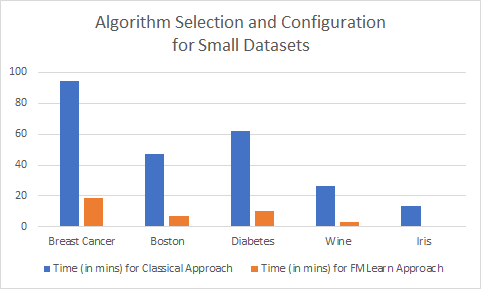
\includegraphics[width=15cm]{images/Small Datasets.png}
    \caption{Execution Time for Small Datasets as seen in Table \ref{table:1}}
    \label{fig:small_dataset}
\end{figure}

Hence, for a small dataset, the user saves an average of 48.79 minutes and about 92.24 minutes (for Breast-Cancer Dataset) in a best case scenario. Whereas, for a large dataset the user saves an average of 533.21 minutes and about 869.74 minutes (for Skin Segmentation Dataset) in a best case scenario. This amounts to about 86.72\% and 95.762\% (for small and large datasets respectively) of time saved for the user, which otherwise is spent waiting for the machine learning program to performs algorithm selection and hyper-parameter optimisation to select the best algorithm-parameters pair for the given dataset. In a scenario where the user would want to re-optimize hyper parameters, re-training was required for only the best algorithm suggested by FMLearn. Under these circumstances, time saved on an average by the user was about 40.864 minutes for small datasets and 513.15 minutes for large datasets. These recommendations for best performing algorithms were consistent with the previously obtained results for the same data and thus reporting a 100\% accuracy for recommendations for previously seen datasets.

\begin{table}[H]
\centering 
\vspace*{+5pt}
 \begin{tabular}{ |p{1.8in}||p{1in}|p{0.7in}|p{1in}|p{0.8in}|  }
 \hline
 \multicolumn{5}{|c|}{Execution Time (in minutes) for Large Datasets} \\
 \hline
 Datasets & Optimize All Algorithms & FMLearn & Re-Optimise best algorithm & Saving in \%\\
 \hline
 Adult & 582.51 & 0.05 & 19.01 & 96.72 \\
 \hline
 MAGIC Gamma Telescope & 279.01 & 0.04 & 14.63 & 94.74 \\
  \hline
 Nursery & 256.42 &  0.04 & 15.47 & 93.95 \\
 \hline
 Skin Segmentation & 869.74 & 0.05 & 29.86 & 96.56 \\
 \hline
 Statlog-Shuttle & 678.37 & 0.04 & 21.35 & 96.84 \\
 \hline
 \hline
 \textbf{Average} & 533.21 & 0.044 & 20.06 & 95.762 \\
 \hline
\end{tabular}
\vspace*{+5pt}
\caption{Execution time when using GridSearch vs FMLearn for large datasets}
\label{table:2}
\end{table}
\vspace*{-10pt}

\begin{figure}[H]
    \centering
    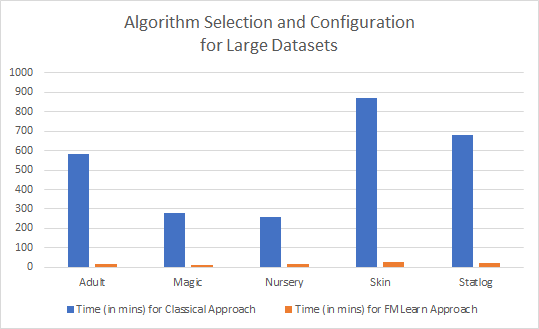
\includegraphics[width=15cm]{images/Large Datasets.png}
    \caption{Execution Time for Large Datasets as seen in Table \ref{table:2}}
    \label{fig:large_dataset}
\end{figure}

%% new page for spacing
\newpage

Figures \ref{fig:small_dataset} and \ref{fig:large_dataset} visually represent and compare the overall time consumed by traditional approach vs FMLearn's approach. From these figures we can see the advantages of using FMLearn over the traditional approach for algorithm selection or other AutoML libraries. FMLearn provides accurate and quick responses by making recommendations from a model created using historic performance data. Since, it is an ever growing and ever learning application, the recommendations made by FMLearn gets better over time. Percentage of Time saved by using FMLearn for small and large datasets are represented in Figure \ref{fig:percentage_time_saved}. Figure \ref{fig:small_dataset_time_Saved} represents the percentage of time saved for small datasets as a radial chart, where each doughnut represents a dataset and the arc length of the doughnut represents the percentage of time saved by the user when using FMLearn. Similarly figure \ref{fig:large_dataset_time_saved} represents the percentage of time saved for a large dataset.

\begin{figure}[H]
\centering
\begin{subfigure}{8cm}
  \centering
  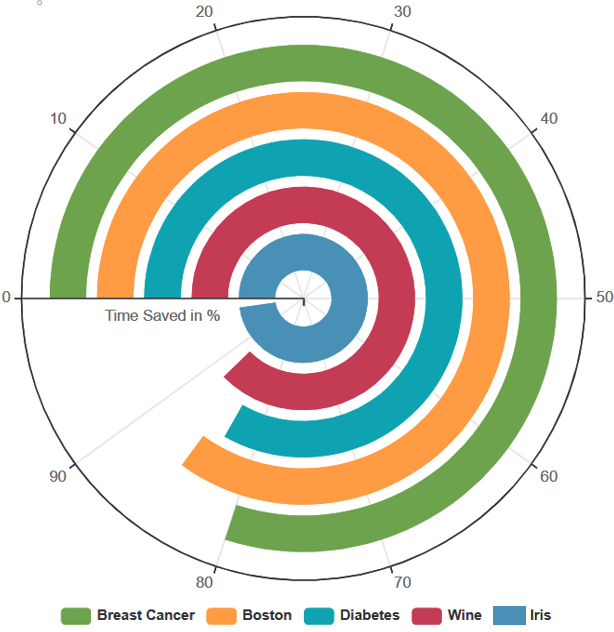
\includegraphics[width=\linewidth]{images/Percetnage Small Datasets.png}
  \caption{Small Dataset}
  \label{fig:small_dataset_time_Saved}
\end{subfigure}%
\begin{subfigure}{8cm}
  \centering
  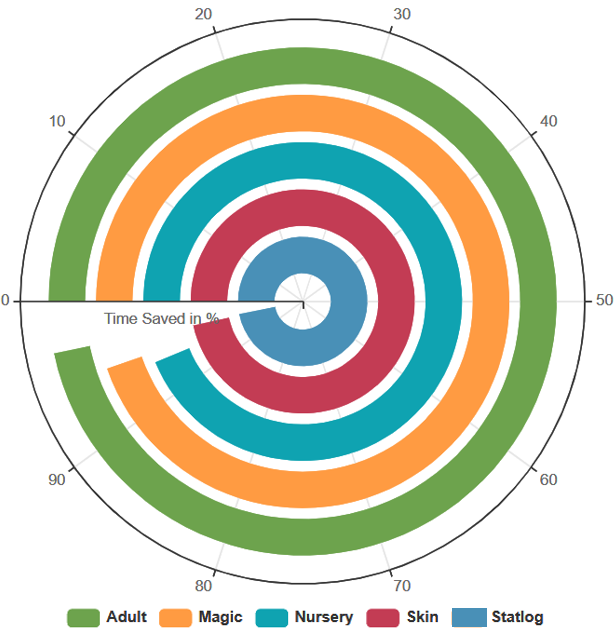
\includegraphics[width=\linewidth]{images/Percentage Large Datasets.png}
  \caption{Large Dataset}
  \label{fig:large_dataset_time_saved}
\end{subfigure}
\caption{Percentage of Time Saved}
\label{fig:percentage_time_saved}
\end{figure}


Upon considering the statistics obtained from the above results and using them in calculating the power consumption, we can see that the average power consumed for finding the best performing algorithm using the traditional approach for one of the small datasets is about 65.061W, but when FMLearn was used the average power consumed is only about 10.629W which is about 86.718\% saving in the power used. In the case of large datasets, the average power consumed to find the best performing algorithm is about 710.946W, but when FMLearn was used the average power consumed is only about 26.805W, which is about 95.762\% reduction in power used when compared to the traditional approach where FMLearn is not used.

\subsection*{Algorithm Recommendations}

Recommending the best algorithm falls into 3 different categories based on the closeness of the input dataset as explained in Section \ref{knn-model}, which can be categorised as follows:
\begin{itemize}
    \item Previously known dataset.
    \item Previously unknown dataset, which is similar to a known dataset.
    \item Previously unknown dataset, which is dissimilar to a known dataset.
\end{itemize}

The results discussed above are for previously known datasets. In the case of unknown but similar datasets, a the same experiment was conducted but with one modification, instead of using an known dataset, unknown yet, similar datasets was used. This similar datasets was obtained from a large dataset like the Statlog-Shuttle dataset. For example this dataset was taken and broken down into small chunks of about 100k records, and these small subsets of data were used to get recommendations from FMLearn. Though the meta-features of the dataset varied, we can be confident that the changes in values will be not drastic as were obtained from the same parent dataset. In this case, the prediction of algorithm is accurate, but the hyper-parameters required re-optimisation to suite the new subset of the data. Whereas, in the case of a previously unseen dataset which is highly dissimilar to the datasets known to FMLearn, the model is able to predict the type of machine learning problem the dataset belongs to, i.e, if it's a classification, regression, clustering, etc, but not the best algorithm for it, it instead recommends a set of algorithms which it thinks are the best in this case instead of recommending a single algorithm. In this case, the best performing algorithm is recommended by FMLearn about 60\% of the time. This set of algorithms are based on the closeness between the previously known datasets.